%!TEX root = ./template-skripsi.tex
%-------------------------------------------------------------------------------
%                            	BAB III
%               		    METODE PENELITIAN
%-------------------------------------------------------------------------------

\chapter{Metode Penelitian}

\section{Desain }

\begin{figure}
  \centering{}
  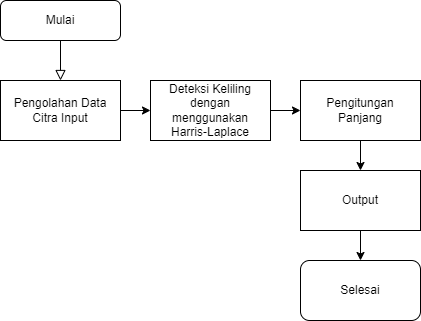
\includegraphics[width=0.45\textwidth]{gambar/Flowchart Penelitian.png}
  \caption{Diagram alur penelitian}
\end{figure}

Sistem yang akan dikembangkan dalam penelitian ini adalah sebuah sistem yang mampu mengukur panjang dan berat dari objek ikan menggunakan metode deteksi Harris-Laplace. 
Fokus utama penelitian ini adalah untuk menghasilkan nilai-nilai panjang dan berat yang terukur dari gambar-foto objek ikan. 
Data set yang akan digunakan dalam penelitian ini akan diperoleh dari internet.
Namun, tidak semua jenis ikan akan digunakan dalam data penelitian ini. 
Penelitian akan berfokus pada dua jenis ikan, yaitu ikan lele dan ikan nila, sebagai data set yang digunakan dalam eksperimen dan pengembangan sistem.


